\documentclass[sigconf, nonacm]{acmart}

\usepackage{tabularx}
\usepackage{makecell}
\usepackage{color,soul}
\usepackage{tablefootnote}
\usepackage{microtype}

\newcolumntype{C}{>{\centering\arraybackslash}X} 

\AtBeginDocument{
  \providecommand\BibTeX{{
    Bib\TeX}}}

\acmConference[LEAK '25]{Unusual Side Channels and Privacy Leaks}{Februrary 07, 2025}{Berlin, Germany}
\setcopyright{cc}
\setcctype[4.0]{by-sa}
\acmDOI{}
\acmISBN{}

\begin{document}

\title{Eavesdropping Speech with Non-sensing Devices}

\author{Tim Holzhey}
\affiliation{
  \institution{Faculty of Electrical Engineering and Computer Science,}
  \institution{Technische Universität Berlin}
  \city{Berlin}
  \country{Germany}
}
\email{holzhey@campus.tu-berlin.de}

\begin{abstract}
  % Topic + Relevance
  In recent years, numerous research papers have shown that sound produced by human speech or other sources can induce minuscule vibrations into a variety of non-acoustic sensors (e.g. motion sensors) or into externally measured objects (e.g. vibrometer) influencing sensor readings in a reversible manner, effectively turning them into undisclosed microphones.
  This allows for eavesdropping on private speech by compromised unsuspicious devices and therefore posing a real threat to privacy when exploited.
  
  % Objective of this paper
  This work will examine and compare different types of vibration-based eavesdropping attacks using a side channel employed on common IoT and smart devices to recover speech or infer privacy-sensitive information about the speaker like their identity, political views, or gender.
  By highlighting notable previous research in this field, we explore the steps necessary to take control of the targeted device, gather the necessary data, and perform signal processing and machine learning techniques to extract audible information from the sensor readings.
  The experimental setups and findings of 16 research papers published in the last decade are compared and discussed, to provide a timeline and trend of the development, limitations, and advancements.
  The overview established over the attacks then allows for a comprehensive feasibility study for the respective attack methods and complexity required to perform such attacks in a real world scenario.
  We discuss possible countermeasures to mitigate the risk of such attacks and provide an outlook on future research directions in the field.
\end{abstract}

\begin{CCSXML}
  <ccs2012>
  <concept>
  <concept_id>10002978.10003001.10010777.10011702</concept_id>
  <concept_desc>Security and privacy~Side-channel analysis and countermeasures</concept_desc>
  <concept_significance>500</concept_significance>
  </concept>
  <concept>
  <concept_id>10002978.10003001.10003003</concept_id>
  <concept_desc>Security and privacy~Embedded systems security</concept_desc>
  <concept_significance>500</concept_significance>
  </concept>
  <concept>
  <concept_id>10010520.10010553.10010559</concept_id>
  <concept_desc>Computer systems organization~Sensors and actuators</concept_desc>
  <concept_significance>500</concept_significance>
  </concept>
  </ccs2012>
\end{CCSXML}

\ccsdesc[500]{Security and privacy~Side-channel analysis and countermeasures}
\ccsdesc[500]{Security and privacy~Embedded systems security}
\ccsdesc[500]{Computer systems organization~Sensors and actuators}

\keywords{Security, Privacy, Side-channel, Eavesdropping, Speech, Acoustic, Hardware Security, Privacy Leaks}

\received{7 January 2025}
% \received[revised]{12 March 2009}
% \received[accepted]{5 June 2009}

\maketitle

\section{Introduction}
The IoT market is on the rise and is still growing exponentially - projected to exceed USD 4 trillion by 2032 \cite{FortuneBusinessInsights2024} - this opens up a new attack vector for adversaries to exploit in addition to traditional software vulnerabilities in computers.
The latest surveys show that American households had on average 21 connected devices \cite{DeloitteConnectedConsumer2023}, of which a significant part are IoT and Smart Home devices.
IoT devices are often equipped with a variety of sensors to interface with their physical environment, such as accelerometers, gyroscopes, microphones, and cameras.
Many of these sensors can also be found on modern smartphones and tablets, which most people carry around\footnote{Surveys from 2024 suggest that 91 \% of Americans own a smartphone \cite{PewResearchMobileFactSheet2024}}. Devices running on \textit{Android} and alike mobile operating systems provide zero-permission access to sensor data from the built-in accelerometer and gyroscope, therefore, have been the subject of the majority of research done in this field.
The findings from vulnerabilities found in smartphones can be projected onto many IoT and smart devices that are equipped with similar sensors but do not have a primary function of audio recording, i.e., do not have a built-in microphone (in that regard "non-sensing").
To execute a vibration-based eavesdropping attack, most of the previous papers took the approach to exploit motion sensors implemented using micro-electromechanical systems (MEMS accelerometers, gyroscopes and magnetometers) commonly found in smartphones and many smart devices like smartwatches, fitness trackers or gaming controllers.
Some of the more experimental approaches have also shown that other sensors like LiDAR scanners in vacuum cleaners, the position error signal of write heads in hard drives, or electro-optical sensors directed at ceiling lights can be exploited for similar attacks.
\\
\begin{sloppypar}
  \noindent
  \textbf{CONTRIBUTION AND LIMITATIONS:} Although a significant part of research done in this field is investigating keystroke recovery attacks \cite{Touchtone2023}\cite{TouchLogger2011}\cite{TapLogger2012}, device fingerprinting \cite{AccelerometerFingerprinting2016}\cite{MEMSFingerprinting2013} or is using sophisticated external setups (e.g. RFID-Tags \cite{RFMic2023}, millimeter-waves \cite{MMMic2022}, WiFi radio \cite{ART2015}), we limit the scope of this paper to \textbf{on-device vibration-based speech and general sound eavesdropping attacks}.
  This includes attacks in theory possible without any modified or additional hardware assuming a compromised device or malicious software.
  This work aims to provide a comprehensive overview of the development and current state of research (SOTA attacks) in the field of vibration-based eavesdropping attacks on non-sensing devices.
  We highlight notable research papers and their findings, compare the different attack methods and achieved results, and discuss the feasibility and possible countermeasures of such attacks in real-world scenarios.
\end{sloppypar}

\section{Background}
\subsection{Vibration-based Eavesdropping Side-Channel Attacks}
Sound created by a human speaking or any other sound can be characterized as spatially and temporally propagating changes in air pressure in the audible frequency range (20 Hz - 20 kHz).
Similarly to how sound waves induce vibrations into our eardrums to let us perceive sound, they can also couple vibrations into all other objects they encounter, more so into objects that are resonant at the frequency of the sound.
In a typical microphone, an oscillating diaphragm is used to convert these vibrations into an electrical signal i.e. a change in voltage by varying the capacitance of the circuit (condenser microphone) or by inducing a current into a coil (dynamic microphone).
Even if unintended, the same phenomenon can be used to turn any other sensing electrical component into a microphone if it has a moving part capable of influencing the electrical properties of the component directly (e.g. MEMS, write head of a hard drive) or observing the spaciotemporal properties of another object (e.g. laser vibrometer, Lidar scanner, camera).
As audible information was not intended to be captured by these sensors, an attacker who is able to recover this information from the sensor readings is exploiting a side channel vulnerability.

\subsection{MEMS}
\begin{sloppypar}
  Sensors manufactured using micro-electromechanical systems (MEMS) incorporate electronics and moving parts on a micrometer-scale chip to measure physical parameters like acceleration (accelerometer), orientation and angular velocity (gyroscope) or the magnetic field (magnetometer).
  The fabrication process makes use of semiconductor manufacturing techniques including lithography and etching on silicon wafers that allows for the production of small, low-cost sensors with high sensitivity and accuracy.
  They are widely used in consumer electronics to enable features like screen rotation, step counting, navigation and gaming feedback.
  On a physical level, MEMS sensors are most commonly realized by a spring-suspended proof mass that changes the capacitance of the circuitry when displaced (variable capacitance MEMS) or by a flexible piezoelectric material that changes its electrical resistance when bent (piezoresistive MEMS).
  The structures can be repeated and aligned in three orthogonal directions to measure the physical property in the three-dimensional spacial domain.
  \vspace{0.25cm}
\end{sloppypar}
\noindent
\textbf{MEMS Accelerometer:} An accelerometer measures the proper acceleration (change in velocity) of an object relative to a local inertial reference frame.
In the gravitational field of the earth, the accelerometer's measurement is offset by the upwards acceleration of 1 g (9.81 m/s\textsuperscript{2}) relative to the free-falling reference frame.
The basic mechanical structure of an accelerometer consists of a damped proof mass suspended by springs that is displaced when the sensor is accelerated in the opposite direction of movement.
In a typical VC MEMS accelerometer, the proof mass moves between air-gapped fixed electrodes forming a variable capacitor as shown in Figure \ref{fig:MEMS_accelerometer}.
\\[6pt]
\textbf{MEMS Gyroscope:} A gyroscope measures the angular velocity (rate of rotation) of an object relative to a local inertial reference frame.
Gyroscopes realized as a MEMS sensor are commonly Vibrating structure gyroscopes (VSG) that measure the Coriolis force acting on a vibrating proof mass when the sensor is rotated.
As the vibrating mass tends to continue vibrating in the same plane, the Coriolis force deflects the mass in the direction perpendicular to the rotation axis.
The deflection is measured by capacitive sensing or piezoresistive sensing and is proportional to the angular velocity of the rotation as shown in Figure \ref{fig:MEMS_gyroscope}.
\\[6pt]
\textbf{MEMS Magnetometer:} A magnetometer measures the strength and direction of the local magnetic field.
MEMS-based magnetometers are often implemented using the Lorentz force acting on the current-carrying conductor in the magnetic field to move the mechanical structure.
The displacement is then measured by capacitive, piezoresistive or optical sensing and is proportional to the magnetic field strength.

\begin{figure}[H]
  \centering
  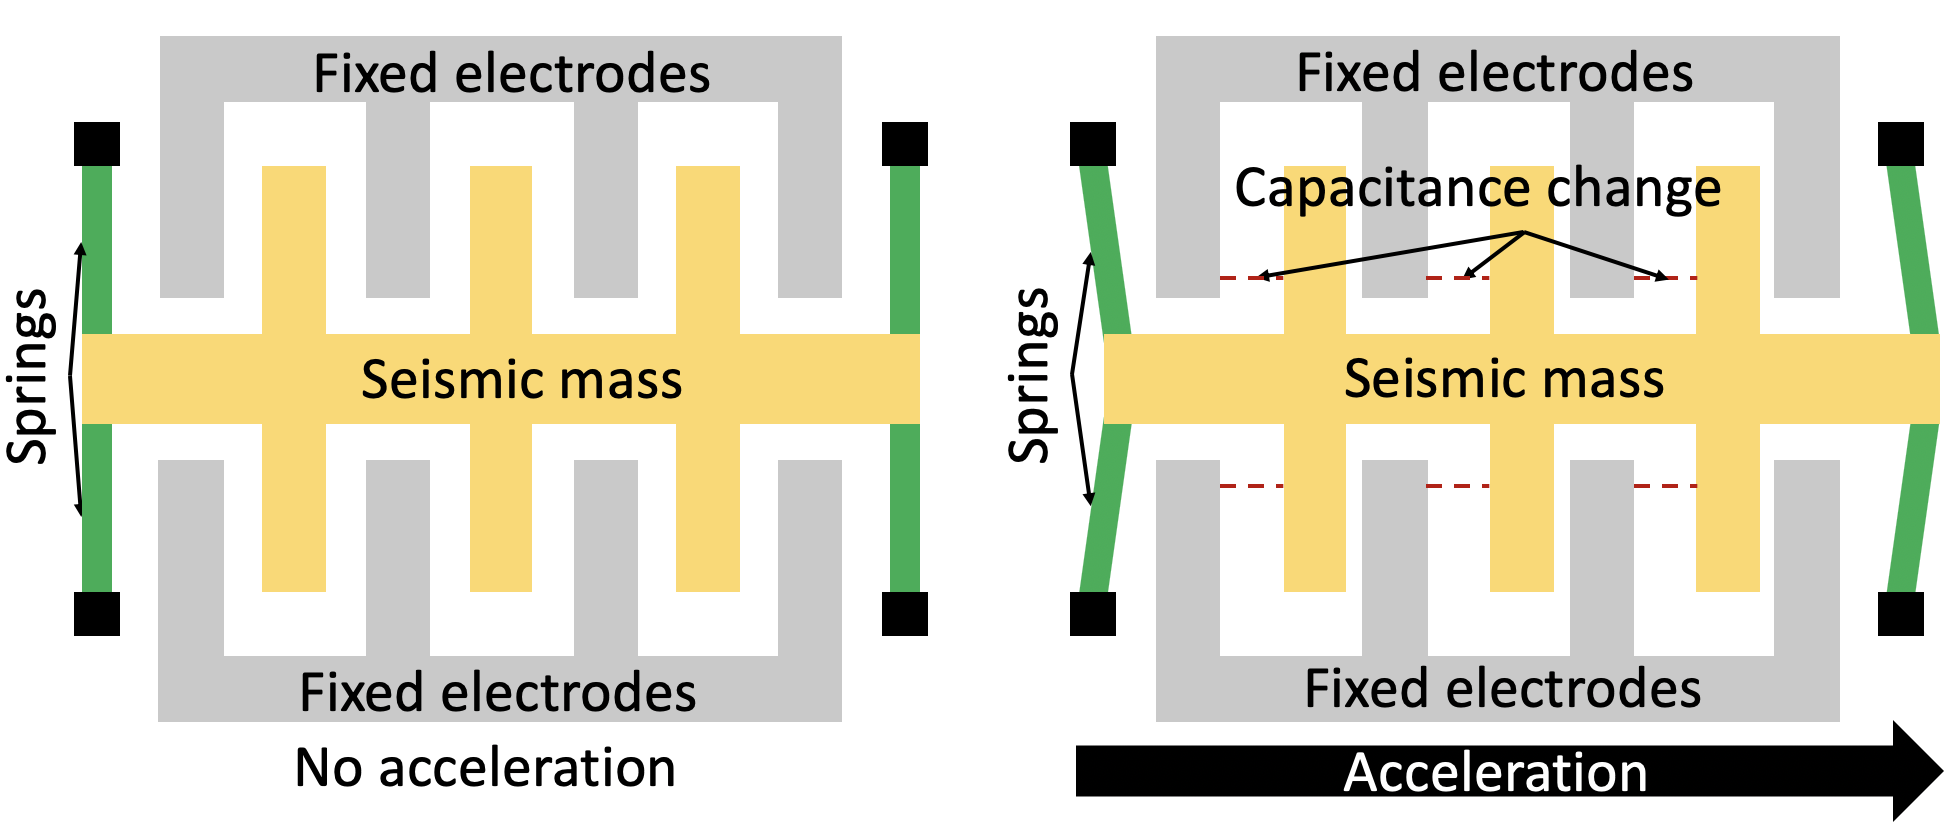
\includegraphics[width=\linewidth]{embed/MEMS_accelerometer.png}
  \caption{Accelerometer - Capacitive MEMS structure, \\Source: \textit{AccelEve} 2020 \cite{AccelEve2020}}
  \Description{Schematic of a MEMS accelerometer structure}
  \label{fig:MEMS_accelerometer}

  \vspace{0.25cm}

  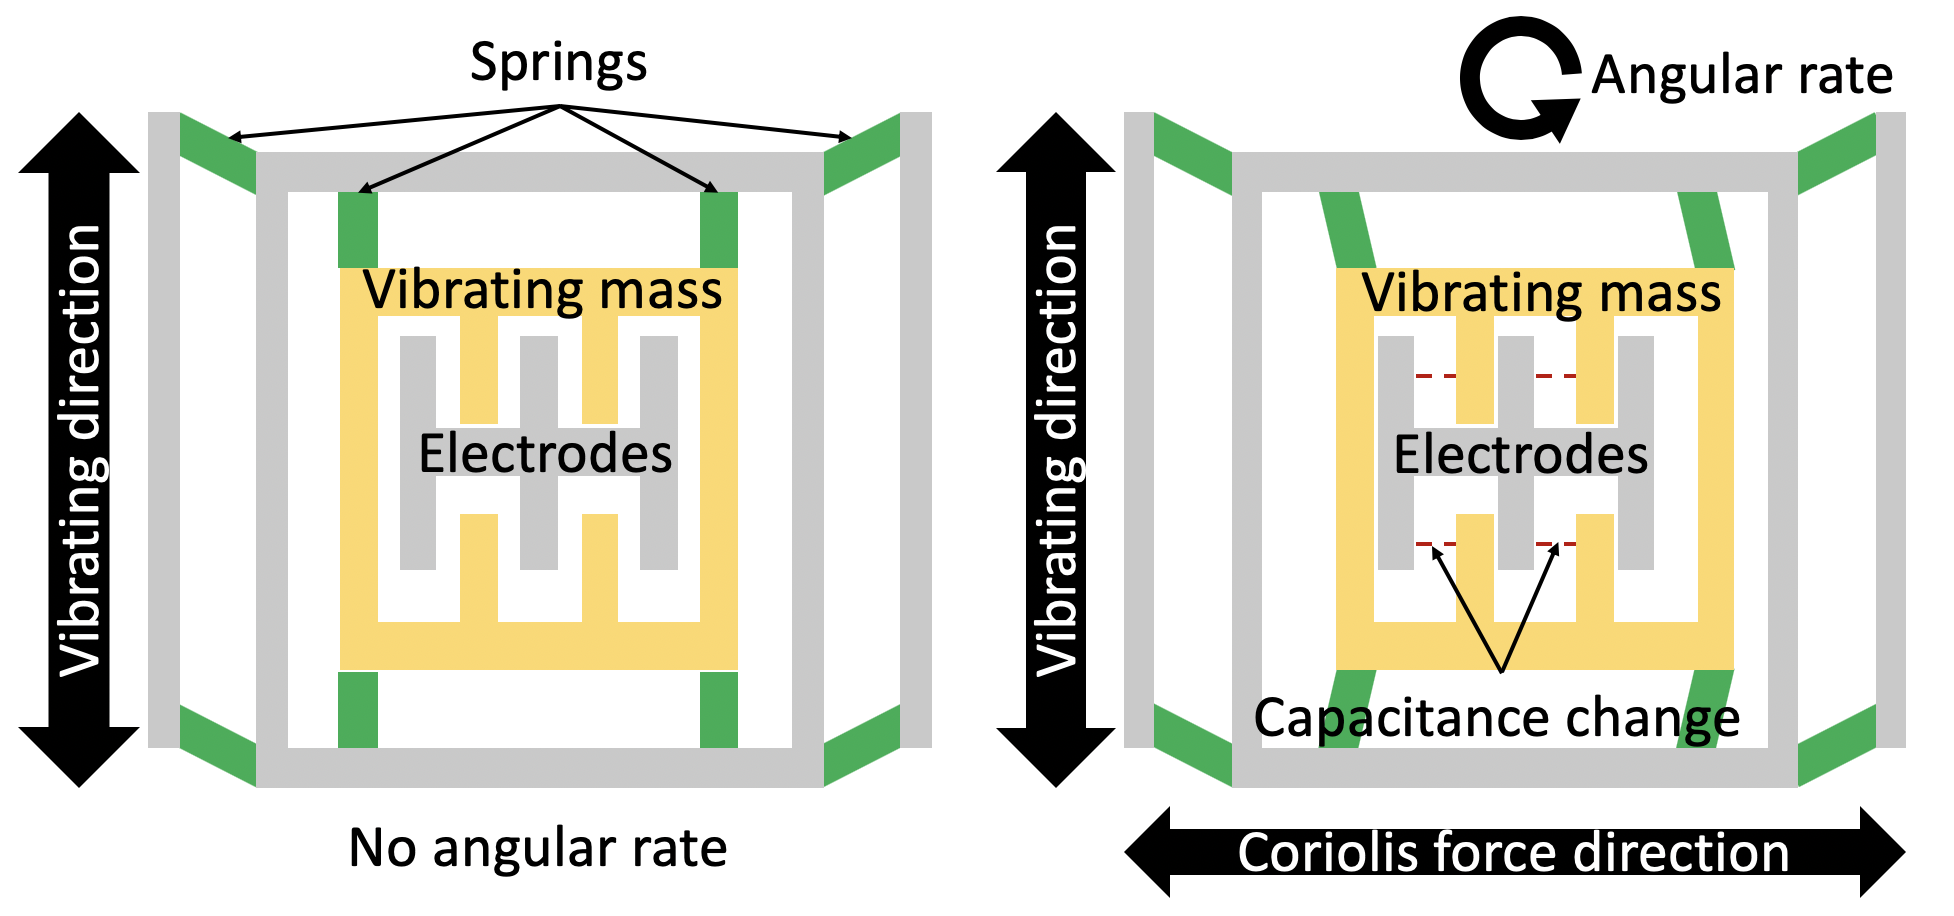
\includegraphics[width=\linewidth]{embed/MEMS_gyroscope.png}
  \caption{Gyroscope - Capacitive MEMS structure, \\Source: \textit{AccelEve} 2020 \cite{AccelEve2020}}
  \Description{Schematic of a MEMS gyroscope structure}
  \label{fig:MEMS_gyroscope}
\end{figure}

\subsection{Laser-based Sensors}

Laser-based measurement devices (e.g. LiDAR scanners, interferometers, vibrometers) are used in various applications to measure precise distances, velocities and material properties contactlessly in various scientific, industrial and medical applications, but recently they made their way into consumer electronics.
Prominently, LiDAR scanners consolidate themselves in our daily lifes as they are increasingly used in applications like autonomous vehicles (Waymo Self-Driving \cite{WaymoDriver}), drones (DJI UAVs \cite{DJIEnterpriseLidar}), robotic vacuum cleaners, \textit{Apple FaceID} or Augumented Reality enabled smartphones.
\\~\\
\textbf{LiDAR Scanner:} LiDAR (Light Detection and Ranging) is a remote sensing and imaging technique that uses a pulsed laser beam to measure the distance to a target object by measuring the time it takes for the light to reflect back to the sensor (Time of Flight) with known speed of light ($d=\frac{c\cdot t}{2}$).
LiDAR systems can map the environment in all directions by rotating the laser beam in a horizontal plane (mechanical spinning LiDAR, Figure \ref{fig:LiDAR}) or by other techniques (solid-state MEMS, optical phased array, Flash LiDAR) and measuring the distance at different angles. The system can be further extended to a 3D LiDAR by adding more vertical scanning layers.
The cummulative distance measurements can be used to create a point cloud representation of the environment.
In order to not interfere with other optical sensors (e.g. camera, human eye), LiDAR's wavelength is mainly located in the near-infrared part of the electromagnetic spectrum (750 nm to 1.5µm).
\\[6pt]
\textbf{Laser Doppler Vibrometer:} A laser microphone uses a laser beam to detect sound vibrations in a distant object. The minute differences in the distance traveled by the light as it reflects from the vibrating object are detected interferometrically. The Laser Doppler Vibrometer (LDV) implements this principle of laser interferometry by splitting the laser into two beams, one of which is reflected off the vibrating object. The surface will module the phase and frequency of the light due to the Doppler effect. One of the beams is passed through a Bragg cell (acousto-optic modulator) to add a frequency shift and then recombined with the other beam to be directed to a photodetector (Figure \ref{fig:LDV}). The electrical signal produced by the photodetector is equal to the carrier frequency produced by the Bragg cell modulated by the Doppler frequency of the vibrating object and proportional to the velocity of the object.

\begin{figure}[H]
  \centering
  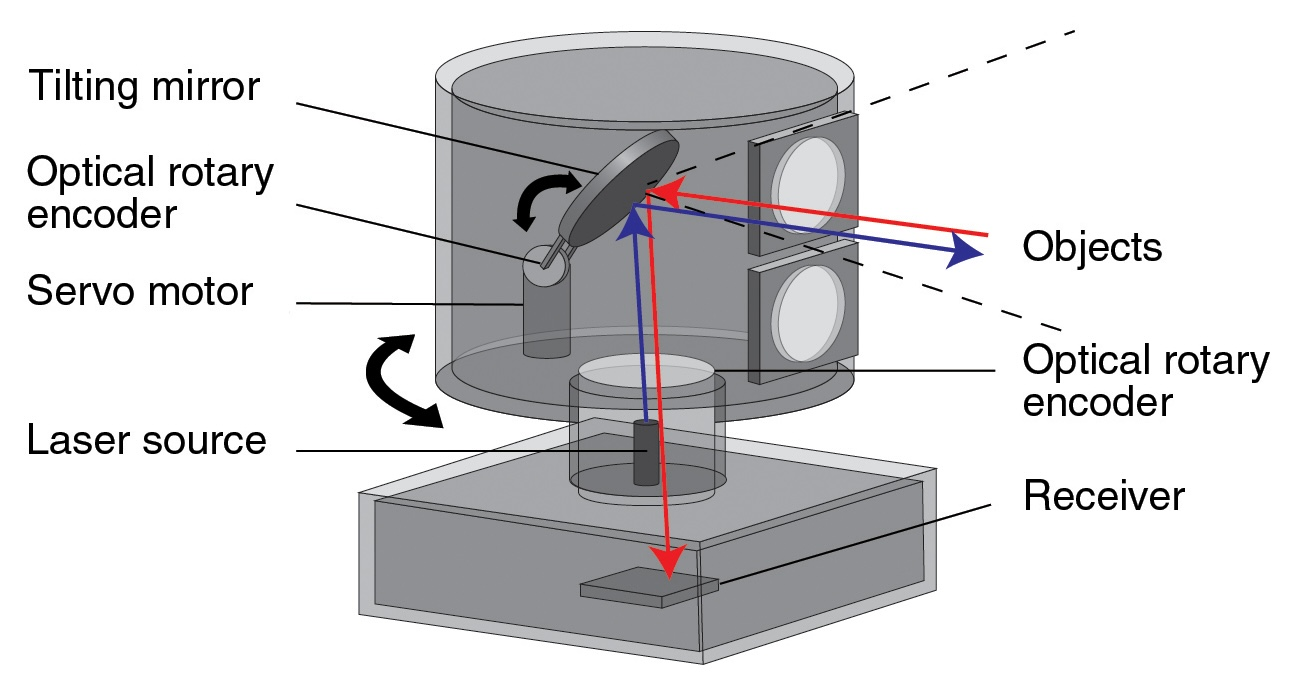
\includegraphics[width=\linewidth]{embed/Lidar_scanner.jpg}
  \caption{Mechanical spinning LiDAR \cite{RenishawLidar}}
  \Description{Schematic of a mechanical spinning LiDAR}
  \label{fig:LiDAR}

  \vspace{0.5cm}

  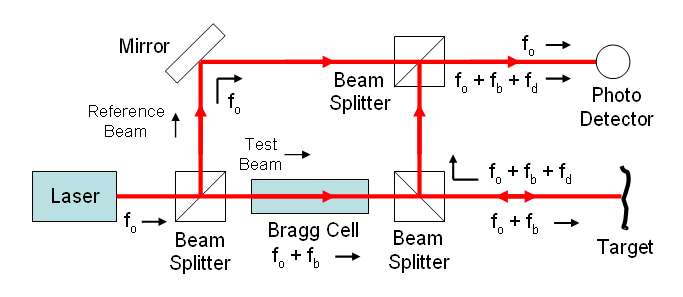
\includegraphics[width=\linewidth]{embed/Laser_Doppler_Vibrometer.png}
  \caption{Laser Doppler Vibrometer \cite{WikipediaLDV}}
  \Description{Schematic of a Laser Doppler Vibrometer}
  \label{fig:LDV}
\end{figure}

\subsection{Speech Intelligibility}
A human speeking in a non-tonal language like English produces a complex waveform that is composed of various frequencies in the audible range.
While the fundamental frequency $f_0$ (lowest frequency component) of the human voice is typically in the range of 100 Hz to 300 Hz (higher for women and children), overtones and consonant articulations can cover most of the audible frequency range of up to 17 kHz (Figure \ref{fig:SpeechFrequencySpectrum}).
Research has shown that frequencies between 1 kHz and 4 kHz are most important for speech intelligibility by surveying with masking band-pass filters \cite{DPAMicrophonesFactsAboutSpeechIntelligibility}.
Applying a low-pass filter to the speech signal at 1 kHz and below quickly degrades the intelligibility of the speech to near zero as perceived by humans (Figure \ref{fig:SpeechIntelligibility}).
Usual digital audio recording and playback systems operate at a sampling rate of 44.1 kHz or 48 kHz to capture the full audible frequency range.
Since most experiments conducted using motion sensors are limited to a sampling rate of 100-500 Hz, machine learning techniques have to be employed to recover (fill in) frequencies above the Nyquist frequency $f_N = \frac{1}{2}f_s$ that are essential for speech intelligibility but not encoded in the sensor readings directly.
For intelligible speech it has been shown, a minimum peak signal-to-noise ratio (PSNR) of 25 - 30 is required \cite{DPAMicrophonesFactsAboutSpeechIntelligibility}.

\begin{figure}[H]
  \centering
  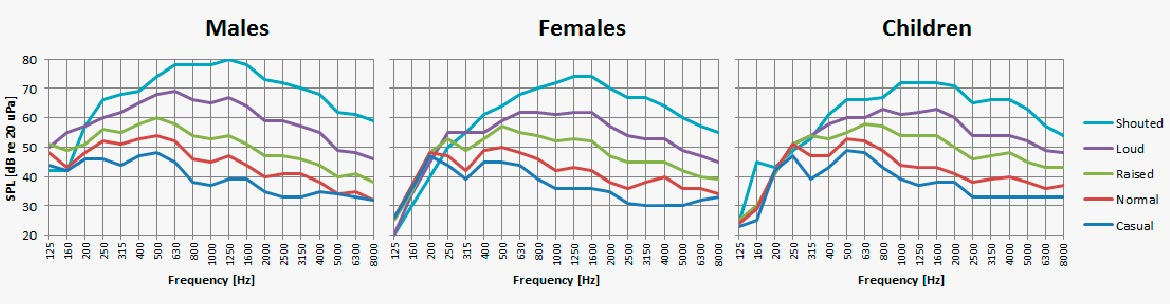
\includegraphics[width=\linewidth]{embed/Speech_frequency_spectrum.jpg}
  \caption{Frequency spectrum of a human voice for Males, Females and Children \cite{DPAMicrophonesFactsAboutSpeechIntelligibility}}
  \Description{Frequency spectrum of a human voice}
  \label{fig:SpeechFrequencySpectrum}

  \vspace{0.5cm}

  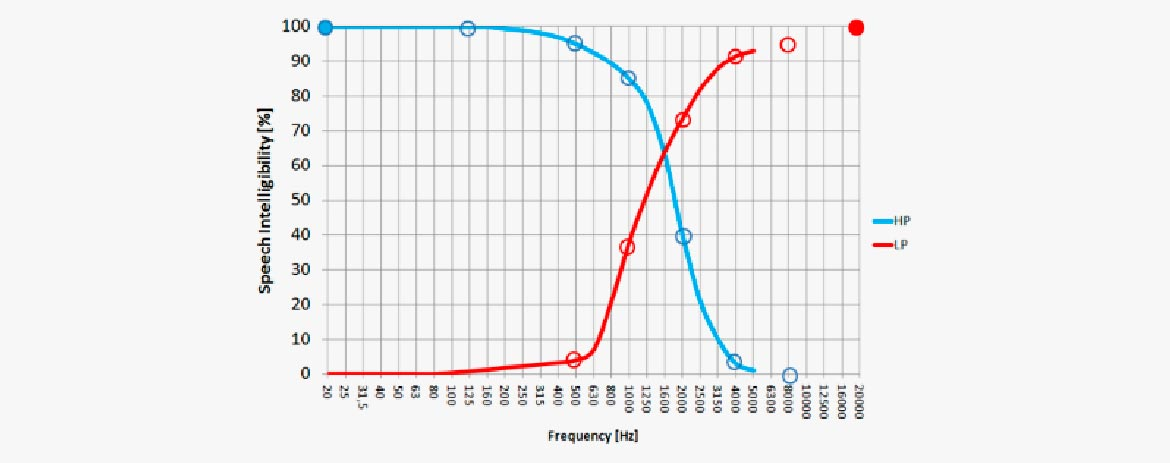
\includegraphics[width=\linewidth]{embed/Speech_Intelligibility_Low_High_Pass_Filter.jpg}
  \caption{Speech intelligibility with low-pass and high-pass filters applied at various frequencies \cite{DPAMicrophonesFactsAboutSpeechIntelligibility}}
  \Description{Speech intelligibility with low-pass and high-pass filters}
  \label{fig:SpeechIntelligibility}
\end{figure}

\section{Literature Review}
\subsection{MEMS-based Eavesdropping Attacks}

Although MEMS sensors are designed to be best insensitive to acoustic noise which would degrade their signal-to-noise ratio, they are still susceptible to sound waves that induce vibrations in the sensor structure.
A MEMS-based eavesdropping attack exploits this vulnerability by recovering the sound-induced vibrations from the sensor readings and reconstructing the original sound.
These types of attacks need to overcome several challenges that include the low sampling rate of the sensors (order of magnitude 100 Hz - 500 Hz), the poor signal-to-noise ratio (PSNR $\ll$ 25) and aliasing artifacts.
\\[6pt]
\textbf{Early Work:} The first paper able to demonstrate the feasibility of recovering speech from motion sensors in typical smartphones was \textit{Gyrophone: Recognizing Speech from Gyroscope Signals} \cite{Gyrophone2014} in 2014 by Yan Michalevsky \textit{et al.}, a joint effort of researchers from Stanford University and the National Research \& Simulation Center (Rafael Advanced Defense Systems Ltd., Isreal).
The authors showed that a smartphone's gyroscope can be used to recover speech rendered by a nearby loudspeaker using sensor readings at a well below Nyquist sampling rate of 200 Hz.
An Android app was developed to record the gyroscope data without requiring any special permissions.
Afterwards, silcence removal and segmentation was applied to the signal that was then fed to the off-the-shelf \textit{Sphinx} speech recognition system to recognize spoken digits of the \textit{TIDIGITS} dataset using spectral statistical features. The authors also trained custom machine learning classifiers (SVM, GMM, DTW) in \textit{Matlab} to identify the speaker and their gender.
With a limited dictionary of spoken english digits (0-9), no assumptions about the speaker and a close distance of 10 cm between the loudspeaker and the smartphone on a solid table surface, a moderate recognition accuracy of at most 26 \% was achieved. Still, they demonstrated speaker classification of up to 50 \% and gender classification of up to 84 \%.
This opened up the field of research to many more papers to come building upon and considerably improving these types of attacks, primarily due to advances in machine learning.
\\~\\
\textbf{Recent Work:} Notably in 2023, Shijia Zhang \textit{et al.} from The Pennsylvania State University leveraged speech eavesdropping attacks using motion sensors in their paper \textit{I Spy You: Eavesdropping Continuous Speech on Smartphones via Motion Sensors} \cite{ISpyU2023} to, for the first time, provide full continuous speech recognition by jointly using accelerometer and gyroscope data.
With a large dictionary of 9950 words and a custom ASR (Automatic Speech Recognition) deep learning model, they achieved 53.3 \% accuracy in recognizing spoken words on an Android smartphone at a sampling rate of 200-500 Hz.
Previously, speech-related attacks were limited to classifying words from a small dictionary (e.g. dataset of 10 spoken english digits) \cite{Gyrophone2014}\cite{Speechless2018}\cite{InertiEAR2022}\cite{VoiceListener2023} or recognizing a single hotword in a stream of words (e.g. dataset of 8 cities) \cite{AccelWorld2015}\cite{AccelEve2020}\cite{Vibphone2021}.

Most recently in 2024, Qingsong Yao \textit{et al.} from Xidian University, China published the paper \textit{Watch the Rhythm: Breaking Privacy with Accelerometer at the Extremely-Low Sampling Rate of 5Hz} \cite{WatchTheRhythm2024} in which they demonstrated that a smartphone's accelerometer can be used for eavesdropping attacks even when limited to a sampling rate of just 5 Hz.
This was achieved by extending the machine learning algorithms to not only consider time-frequency features (spectral) but also the temporal dynamics of the signal (pause rhythm and energy intensity rhythm) that are much better preserved in the very-low frequency domain.
To benchmark against previous papers, the authors showed that english spoken digits could be recognized with an accuracy of 32.70 \% at 5 Hz with an on-device Android app reading accelerometer data (77.79 \% at 200 Hz).
Similar tests to determine typical places like bar, metro, bus and car yielded an average accuracy of 91.28 \%.

\subsection{Laser-based Eavesdropping Attacks}

\textbf{Recent Work:} In 2020, a group of researchers from the University of Singapore and the University of Maryland sparked the interest of the security research community \cite{BitdefenderRobotVacuumEavesdrop} and news outlets \cite{ForbesRobotVacuumEavesdrop} with their paper \textit{Spying with Your Robot Vacuum Cleaner: Eavesdropping via Lidar Sensors} ("LidarPhone") \cite{LidarPhone2020}. A method is introduced that repurposes lidar sensors in robot vacuum cleaners to function as laser-based microphones capable of capturing sound signals by detecting subtle vibrations in nearby objects (Figure \ref{fig:LidarphoneSetup}).
After reverse-engineering and modifying the firmware of a commercial robot vacuum cleaner (Xiaomi Roborock S5) to gain access to the raw lidar data, the authors tricked the device into activating the scanner without rotating its mirror and unknowingly duplicating the sensor data stream to be sent over the local network. Therefore, they could increase the sampling rate of a single point from 5 Hz to 1.8 kHz and later process the data on a remote computer offline.
The robot's lidar scanner was aimed at different kinds of common household objects (e.g. trash can, cardboard box, plastic bag) and sounds were played back from a nearby loudspeaker.
With an array of preprocessing steps (DC-offset correction, outlier removal, interpolation, normalization, high-pass filter, noise removal and equalization) the small signal-to-noise ratio of the sensor readings could be overcome and the authors were able to successfully identify spoken digits, the speaker's identity and gender and music snippets from popular news channels introductory jingles with accuracies of 91 \%, 67.5 \%, 96 \% and 90 \% respectively using classifying and correlating convolutional neural networks (CNN).

\begin{figure}[H]
  \centering
  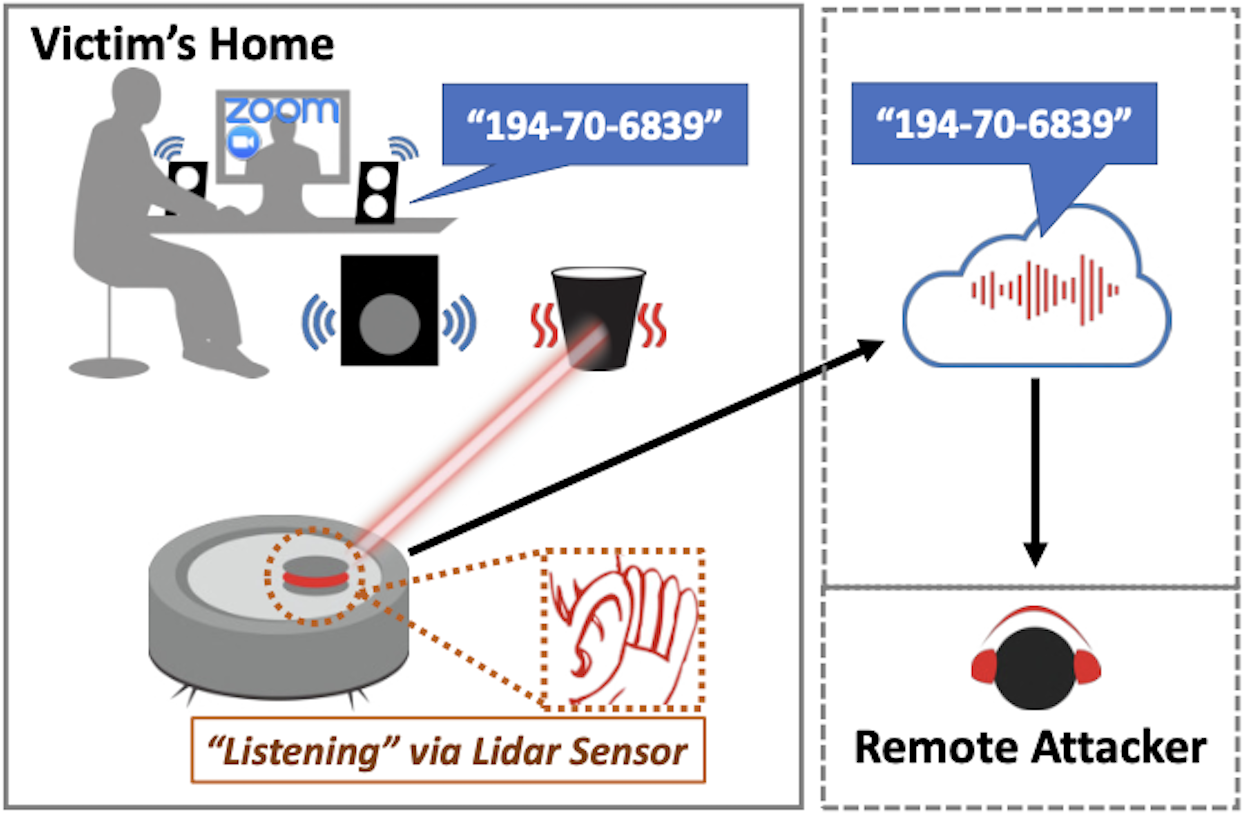
\includegraphics[width=\linewidth]{embed/Lidarphone_setup.png}
  \caption{Experimental setup of the \textit{LidarPhone} attack \cite{LidarPhone2020}}
  \Description{Frequency spectrum of a human voice}
  \label{fig:LidarphoneSetup}
\end{figure}

\subsection{Other Eavesdropping Attacks}

Other notable vibration-based speech eavesdropping side channel attacks explore methods to turn computer hardware and household objects into microphones.

The paper \textit{Hard Drive of Hearing: Disks that Eavesdrop with a Synthesized Microphone} (2019) \cite{HardDriveOfHearing2019} by Andrew Kwong \textit{et al.} from the University of Michigan and Zhejiang University demonstrated that the position error signal (PES) of the read/write head in a hard drive can be used to recover sound signals if subjected to sound vibrations.
Although not exposed to the user, if the hard drive controller's firmware is compromised, the high-fidelity PES (16-bit, 34.56 kHz) can fully encode the recorded sound signal without the need for machine learning assistance. The authors put their experimental microphone to the test by reliably detecting music played from a nearby smartphone with the \textit{Shazam} music recognition app fed with the recorded and processed PES data.

Other noteworthy research has focused on recovering speech with an electro-optical sensor directed at a ceiling light through a telescope (\textit{Lamphone} \cite{Lamphone2022}) which is not further discussed here.

\begin{table*}[ht]
  \caption{Test parameters and key results from a timeline of previous publications on vibration-based speech eavesdropping attacks exploiting different sensors and devices}
\label{tab:PapersParametersComparison}
\scriptsize
\renewcommand{\arraystretch}{1.3}
\begin{tabularx}{\textwidth}{@{} |lp{2.0cm}|CCCCCCCC|X| @{}}
\toprule
\textbf{Year} & \textbf{Paper} & \textbf{Sensor} & \textbf{Measuring Device} & \textbf{Attack Goal} & \textbf{Sampling Freq.} & \textbf{Audio source} & \textbf{Transmission Medium} & \textbf{Distance from source} & \textbf{Dictionary Size} & \makecell{\textbf{Speech Rec.}\\\textbf{(best)}} \\
\hline\hline
2014 & Gyrophone \cite{Gyrophone2014} & Gyroscope & Android Smartphone & Speech Rec., Speaker Ident., Gender Ident. & 200 Hz & External Loudspeaker & Solid Surface & 10 cm & 10 digits & 26 \% \\ \hline
2015 & AccelWorld \cite{AccelWorld2015} & Accelerometer & Android Smartphone & Speech Rec., Speaker Ident. & 200 Hz & External Loudspeaker & Air & 30 cm & 1 hotword & 85 \% \\ \hline
2017 & PitchIn \cite{PitchIn2017} & Accelerometer, Gyroscope, Geophone & Dedicated IMCU & Speech Rec. & 1 kHz & Human & Air & 1 m & 10 words & 79 \% \\ \hline
2018 & Speechless \cite{Speechless2018} & Accelerometer, Gyroscope & Android Smartphone & Speech Rec. & 200 Hz & External Loudspeaker & Solid Surface & 10 cm & 10 digits & 0 \% \\ \hline
2019 & Kinetic Song Comprehension \cite{KineticSongComprehension2019} & Accelerometer, Gyroscope & Android Smartphone & Song Rec. & 100 Hz & Smartphone Loudspeaker & Solid Surface & On-Device & 100 songs & 80 \% \\ \hline
2020 & AccelEve \cite{AccelEve2020} & Accelerometer & Android Smartphone & Speech Rec., Speaker Ident. & 100-500 Hz & Smartphone Loudspeaker & Solid Surface & On-Device & 8 hotwords,\par 36 alphanum. & 90 \% (hotwd),\par 55 \% (alnum),\par 78 \% (digits) \\ \hline
2021 & Spearphone \cite{Spearphone2021} & Accelerometer & Android Smartphone & Speech Rec., Speaker Ident., Gender Ident. & 120-500 Hz & Smartphone Loudspeaker & Solid Surface & On-Device & 10 digits,\par 58 words & 67 \% (words),\par 71 \% (digits)\\ \hline
2021 & Vibphone \cite{Vibphone2021} & Accelerometer & Android Smartphone & Speech Rec. & 225-425 Hz & Smartphone Loudspeaker & Solid Surface & On-Device & 10 hotwords + 10 digits & 54.2 \% \\ \hline
2022 & AccMyrinx \cite{AccMyrinx2022} & Accelerometer & Android Smartphone & Speech Rec. & 100-500 Hz & Smartphone Loudspeaker & Solid Surface & On-Device & Synthesis & 42.7 \% SWER\footnote{Smoothed Word Error Rate} \\ \hline
2022 & InertiEAR \cite{InertiEAR2022} & Accelerometer, Gyroscope & Smartphone & Speech Rec. & 40-200 Hz & Smartphone Loudspeaker & Solid Surface & On-Device & 10 digits & 78.8 \% \\ \hline
2023 & ISpyU \cite{ISpyU2023} & Accelerometer, Gyroscope & Android Smartphone & Automatic Speech Rec. & 200-500 Hz & Smartphone Loudspeaker & Solid Surface & On-Device & 9950 words,\par 2000 words & 53.3 \% (big),\par 59.9 \% (small)\\ \hline
2023 & VoiceListener \cite{VoiceListener2023} & Accelerometer, Gyroscope, Magnetometer & Android Smartphone & Speech Rec. & 100-500 Hz & Smartphone Loudspeaker & Solid Surface & On-Device & 10 digits,\par 10 sentences & 82.7 \% (digits)\par 10 \% (senten)\\ \hline
2023 & StealthyIMU \cite{StealthyIMU2023} & Accelerometer & Android Smartphone & Speech Rec. (Voice Assistant) & 100-500 Hz & Smartphone Loudspeaker & Solid Surface & On-Device & 23 voice commands & 8.46 \% SEER\footnote{Single Entity Error Rate} \\ \hline
2024 & Watch the Rhythm \cite{WatchTheRhythm2024} & Accelerometer & Android Smartphone & Speech Rec., Scene Rec. & 5-200 Hz & Smartphone Loudspeaker & Solid Surface & On-Device & 10 dig. (en+ch),\par 28 scenes,\par 30 cities & 51 \% (dig-en),\par 47 \% (dig-ch),\par 78.7 \% (scene),\par 58.7 \% (cities)\\
\hline\hline
2020 & LidarPhone \cite{LidarPhone2020} & Lidar Scanner & Robot Vacuum Cleaner & Speech Rec., Song Rec., Speaker Ident., Gender Ident. & 1.8 kHz & External Loudspeaker & Air & 1.5 m & 10 digits,\par 10 snippets & 91 \% (digits),\par 90 \% (snippets) \\
\hline\hline
2019 & Hard Drive of Hearing \cite{HardDriveOfHearing2019} & Hard Drive PES & HDD Controller & Speech Rec., Song Rec. & 34.56 kHz & External Loudspeaker & Air & 25 cm & - & Verified,\par no metric \\
\bottomrule
\end{tabularx}
\end{table*}

\section{Feasibility Study}
\begin{sloppypar}
  In the following, 16 of the most cited research papers on device-local vibration-based speech eavesdropping attacks exploiting different sensors and devices published between 2014 and 2024 are compared giving comprehensive insight over the research done in the field from its early pioneers to the very recent advances \cite{Gyrophone2014}\cite{AccelWorld2015}\cite{PitchIn2017}\cite{Speechless2018}\cite{KineticSongComprehension2019}\cite{AccelEve2020}\cite{Spearphone2021}\cite{Vibphone2021}\cite{AccMyrinx2022}\cite{InertiEAR2022}\cite{ISpyU2023}\cite{VoiceListener2023}\cite{StealthyIMU2023}\cite{WatchTheRhythm2024}\cite{LidarPhone2020}\cite{HardDriveOfHearing2019}.
  The test parameters used in the experimental setups of the papers and the key results the authors could achieve (metric for best speech recognition accuracy) are compiled in Table \ref{tab:PapersParametersComparison} in chronological order of publication grouped by the type of sensor the data was collected from.
  Most work focus on MEMS-based attacks using accelerometers, gyroscopes and magnetometers in zero-permission Android or HarmonyOS smartphones, while two papers explore high-fidelity laser-based and miscellaneous attacks for comparison.
\end{sloppypar}
It can be observed that attacks using sensors in smartphones are heavily restricted by the low sampling rate, usually in the realm of 100-500 Hz.
This value is inherently hardware-bound by the sensor circuitry and hardware access overhead, and often times deliberately limited by the operating system to prevent privacy breaches as well as excessive power consumption.
Still, many papers have shown that strikingly high speech recognition accuracies can be achieved with very low sampling rates.
The development towards using larger word dictionaries (9950 words \cite{ISpyU2023}), using a combination of different sensors in conjunction (ACC x GYRO \cite{InertiEAR2022}), proving the privacy concerns still exist with even lower sampling rates (5 Hz \cite{WatchTheRhythm2024}) and experimenting with more sophisticated processing and machine learning pipelines is evident over the years.
Noteworthy is also the achievement of continuous speech recognition in 2023 by \textit{ISpyU} \cite{ISpyU2023} with more than 50 \% word accuracy and almost 10 thousand distinct recognizable words.

\subsection{Limitations}
The results from previous research all mention that the extremely low signal-to-noise ratio (low amplitude signal in relation to sensor noise) is a limiting factor.
To produce meaningful speech recognition the sound-producing source (generally a loudspeaker or subwoofer with 70+ dB) needs to be close and well sound-conducted to the sensor over a solid surface.
In many cases the speaker even shares the same housing with the sensor e.g. in the case of a smartphone that shares both components on one PCB (< 10 cm copper and resin).
Comparative studies have shown accelerometers pick up sounds significantly better than gyroscopes \cite{AccelEve2020} because sound waves generally produce linear acceleration in the direction of travel rather than angular velocity.
The detailed meta analysis conducted in \textit{SoK: Assessing the Threat Potential of Vibration-based Attacks against Live Speech using Mobile Sensors} \cite{SokVibration2021} by Payton Walker \textit{et al.} assessing the real-world thread potential of some of the here mentioned attack methods concludes that the likelihood of a successful attack is fairly low due to the many limiting factors and the need for a controlled testing environment with favorable conditions.

\section{Countermeasures}
In the following, we will discuss possible countermeasures to mitigate the risk of vibration-based eavesdropping attacks on non-sensing devices.

\subsection{Limit Sensor Quality}
One way to lower the success rate of speech recovery attacks is to limit quality metrics of the sensor data exposed to the user.
This can be achieved by reducing the sampling rate of the sensors further (e.g. to 50 Hz), lowering the resolution (bit depth) or by worsening the signal-to-noise ratio deliberately.
However, this would also degrade the performance of the device's primary function and user experience (e.g. slower response to phone rotation in mobile games, aliasing artifacts in video stabilization or faults in lidar mapping).

In the past, mobile operating systems have updated their APIs to limit the sampling rate of motion sensors to 200 Hz (Android \cite{AndroidDeveloperSensorDocs}) and 100 Hz (iOS \cite{AppleDeveloperAccelerometerData}\cite{AppleDeveloperGyroscopeData}) in response to privacy concerns.
While substantially limiting malicious apps from recording high-fidelity audio with motion sensors, research has shown that speech still can be leaked at very low sampling rates (e.g. 5 Hz \cite{WatchTheRhythm2024}) to some extent.

Smartphone sensors are also exposed to web applications by the \textit{Sensor Web API} \cite{MDNWebDocsSensorAPI} available in many modern web browsers (Chrome, Edge, Opera).
The World Wide Web Consortium (W3C) has acknowledged the privacy concerns of exposing raw inertial sensor data to the web content and have proposed an \textit{Accelerometer reading quantization algorithm} \cite{W3CAccelerometerQuantization} that limits the resolution of the accelerometer's XYZ data points to a fixed $0.1 m/s^2$ granularity that is still sufficient for many practical applications.
The W3C Editor's Draft \cite{W3CAccelerometerQuantization} reads:
\begin{quote}
  \vspace{0.1cm}
  \textbf{§ 4. Security and Privacy Considerations} \\
  Sensor readings provided by inertial sensors, such as accelerometer, could be used by adversaries to exploit various security threats, for example, keylogging, location tracking, fingerprinting and user identifying.
\end{quote}

\subsection{Constrain Sensor Access}
Another way to lower the chance of a malicious app recording audio with motion sensors is to further constrain the access to the sensor data.
While iOS is already strictly enforcing obligatory prompts for developers that tell the user why the app is requesting access to the device's motion data (iOS 7.0+ NSMotionUsageDescription \cite{AppleDeveloperMotionUsageDescription}), Android is granting sensor access to apps by default for up to 200 Hz. Apps need to declare the \textit{HIGH\_SAMPLING\_RATE\_SENSORS} permission only to be able to sample the device's accelerometer, gyroscope, and geomagnetic field sensor at higher rates (Android 12+ \cite{AndroidDeveloperSensorDocs}).
Since Android 9 apps also cannot access sensors when running in background and users are able to manage permission preferences for each app individually in the settings.
Google has acknowledged the privacy concerns of sensor-based eavesdropping attacks in the Android Developer's documentation \cite{AndroidDeveloperSensorDocs} by linking sensor rate-limiting to the microphone access:
\begin{quote}
  \vspace{0.1cm}
  \textbf{Sensor Rate-Limiting} \\
  {[\ldots]} \\
  \textbf{Note:} If the user turns off microphone access using the device toggles, the motion sensors and position sensors are always rate-limited, regardless of whether you declare the HIGH\_SAMPLING\_RATE\_SENSORS permission.
\end{quote}

\noindent
IoT devices should also introduce strict hardware-interlocks that e.g. would have prevented the robot vacuum cleaner' LiDAR investigated in \textit{LidarPhone} \cite{LidarPhone2020} from being activated without rotating the mirror.

\subsection{Minimize Acoustic Coupling}
Motion sensors are designed to minimize the acoustic coupling to the sensor structure.
This can be achieved by isolating the sensor from the sound source (e.g. by using a soundproof casing) or by damping the sensor structure in its embedding (e.g. by using dampening pads around the sensor's suspension).
Other proposals include acoustic masking by e.g. introducing white noise into the sensor or band-pass filtering the sensor readings to remove speech-relevant frequencies.

\subsection{Preprocess Audio Data}
Recently, the authors of \textit{EveGuard: Defeating Vibration-based Side-Channel Eavesdropping with Audio Adversarial Perturbations} \cite{EveGuard2024} proposed a software-driven defense mechanism which protects voice privacy by introducing adversarial perturbations into the audio signal produced by a loudspeaker.
They develop a perturbation generator model (PGM) that effectively suppresses sensor-based eavesdropping by introducing inaudible distortions while maintaining high audio quality using machine learning techniques.
This audio preprocessing step could be integrated into smartphones, effectively reducing the ability of the motion sensors to recover sound from the speaker-induced vibrations.

\subsection{Software Security}
Since all eavesdropping attacks previously discussed require the attacker to have control over the device or to have installed malicious software on the device, manufacturers and developers need to actively design their software and firmware to be secure against unauthorized access.
For embedded and IoT devices, this concerns implementing mechanisms like secure boot, signed firmware update, encrypted data storage and locked-down debug interfaces.
Operating systems offering app stores should also enforce strict security policies for apps that request access to sensitive data like motion sensor data.
Special attention should be given to the Android platform, as it is possible to side-load apps from third-party sources without the need to be verified by the Google Play Protect service. The Android OS is globally being used by the vast majority of smartphones and tablets (market share of 73.52 \% in 12/2024 \cite{StatcounterOSMarketShare}) and is therefore a prime target for malicious software.

\section{Conclusion}
In this work, we have provided a comprehensive overview of the state-of-the-art research in the field of vibration-based speech eavesdropping attacks using non-acoustic sensors.
We have highlighted notable research papers and their findings, compared the different attack methods and achieved results, and discussed the feasibility and possible countermeasures of such attacks in real-world scenarios.
The findings show that speech recovery is likely to be very limited in real-world environments due to multiple restricting factors including very low sampling rates, poor signal-to-noise ratios, the need for close proximity to the sound source and solid sound-conducting transmission medium.
Fortunately for the users, no large-scale privacy breach of this kind has been reported to have been exploited in real-world applications yet.
However, analysis show indications of a trend in research to overcome these limitations by using more sophisticated machine learning techniques, sensor fusion and temporal dynamics in conjunction with spectral features.
Although limited, the risk of eavesdropping attacks is still present and manufacturers, developers and users should be made aware of the potential threat and take appropriate countermeasures to protect their privacy looking forward.

%%
%% The acknowledgments section is defined using the "acks" environment
%% (and NOT an unnumbered section). This ensures the proper
%% identification of the section in the article metadata, and the
%% consistent spelling of the heading.
% \begin{acks}
% To Robert, for the bagels and explaining CMYK and color spaces.
% \end{acks}

%%
%% The next two lines define the bibliography style to be used, and
%% the bibliography file.
\bibliographystyle{ACM-Reference-Format}
\bibliography{references}


%%
%% If your work has an appendix, this is the place to put it.
% \appendix

\end{document}
\endinput
%%
%% End of file `sample-sigconf.tex'.
